\subsubsection*{\underline{\textsc{\Large Wight}}}
\noindent\emph{Medium undead, neutral evil}

Wights are intelligent undead humanoids that resemble armed and armored corpses. They never tire in pursuit of their goal of making eternal war against the living.

\noindent\rule{0.5\textwidth}{0.5pt}

\noindent\textbf{Armor Class}: 14

\noindent\textbf{Hit Points}: 45 (6d8 + 18)

\noindent\textbf{Speed}: 30 ft.

\noindent\rule{0.5\textwidth}{0.5pt}
\begin{table}[H]
	\begin{tabular}{cccccc}
		\textbf{STR} & \textbf{DEX} & \textbf{CON} & \textbf{INT} & \textbf{WIS} & \textbf{CHA} \\
		15 (+2) & 14 (+2) & 16 (+3) & 10 (+0) & 13 (+1) & 15 (+2) \\
	\end{tabular}
\end{table}
\noindent\rule{0.5\textwidth}{0.5pt}

\noindent\textbf{Skills}: Perception +3, Stealth +4

\noindent\textbf{Damage Resistances}:  necrotic; bludgeoning, piercing, and slashing from nonmagical attacks that aren't silvered

\noindent\textbf{Damage Immunities}: poison

\noindent\textbf{Condition Immunities}: exhaustion, poisoned

\noindent\textbf{Senses}: darkvision 60 ft., passive Perception 13

\noindent\textbf{Languages}: the languages it knew in life

\noindent\textbf{Challenge}: 3 (700 XP)

\noindent\rule{0.5\textwidth}{0.5pt}

\noindent\textbf{Sunlight Sensitivity}: While in sunlight, the wight has disadvantage on attack rolls, as well as on Wisdom (Perception) checks that rely on sight.

\noindent\rule{0.5\textwidth}{0.5pt}

\noindent\textbf{ACTIONS}

\noindent\textbf{Multiattack}: The wight makes two longsword attacks or two longbow attacks. It can use its Life Drain in place of one longsword attack.

\noindent\textbf{Life Drain}:  Melee Weapon Attack: +4 to hit, reach 5 ft., one creature. Hit: 5 (1d6 + 2) necrotic damage. The target must succeed on a DC 13 Constitution saving throw or its hit point maximum is reduced by an amount equal to the damage taken. This reduction lasts until the target finishes a long rest. The target dies if this effect reduces its hit point maximum to 0. A humanoid slain by this attack rises 24 hours later as a zombie under the wight's control, unless the humanoid is restored to life or its body is destroyed. The wight can have no more than twelve zombies under its control at one time.

\noindent\textbf{Longbow}: Ranged Weapon Attack: +4 to hit, range 150/600 ft., one target. Hit: 6 (1d8 + 2) piercing damage.

\noindent\textbf{Longsword}:  Melee Weapon Attack: +4 to hit, reach 5 ft., one target. Hit: 6 (1d8 + 2) slashing damage, or 7 (1d10 + 2) slashing damage if used with two hands.

\begin{center}
	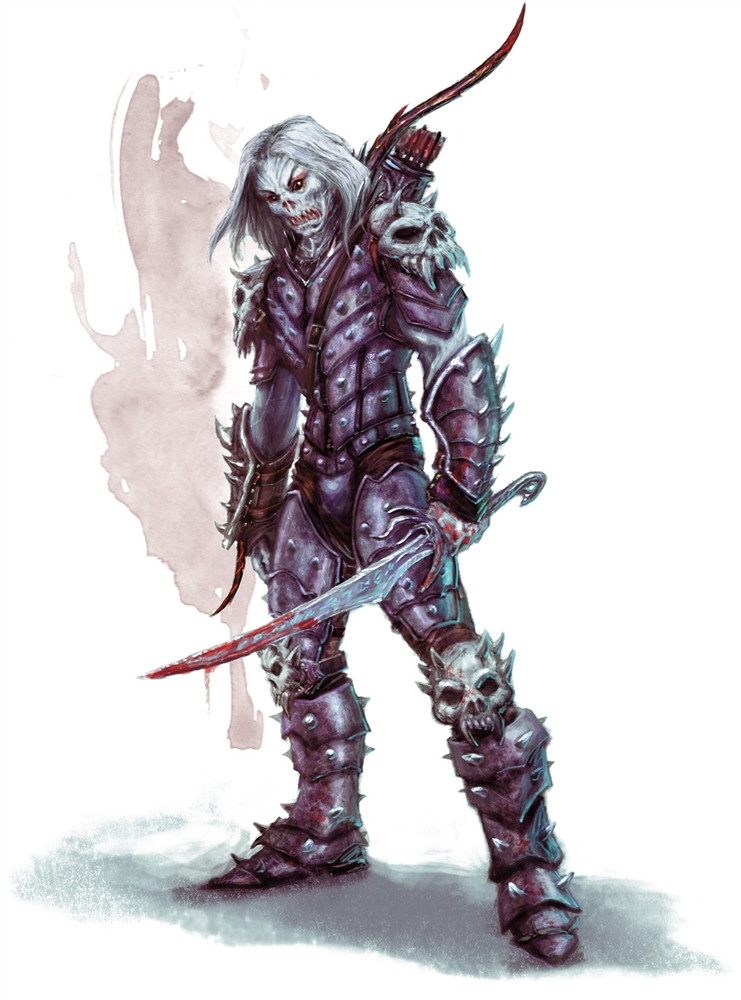
\includegraphics[width = 0.3\textwidth]{wight}
	
	\emph{Wight}
\end{center}